% Copyright 2009--2010  Ed Bueler

\section{shallow ice sheets}

\subsection{solving the SIA}

\begin{frame}{similarity solution to the SIA}

\begin{itemize}
\item jump forward to 1981 \dots breaking news: \quad P.~Halfar finds the fundamental solution of the SIA! \quad [Halfar, 1981; 1983]
\item when $n=3$, Halfar's 2D solution for Glen flow law has scalings
   $$H(t,r)=t^{-1/9} \phi(s), \qquad s = t^{-1/18} r$$
\item \dots therefore, if an ice sheet starts steep and it flows without additional accumulation then its thinning \emph{really} slows down as the shape flattens out
\end{itemize}

\medskip
\begin{center}
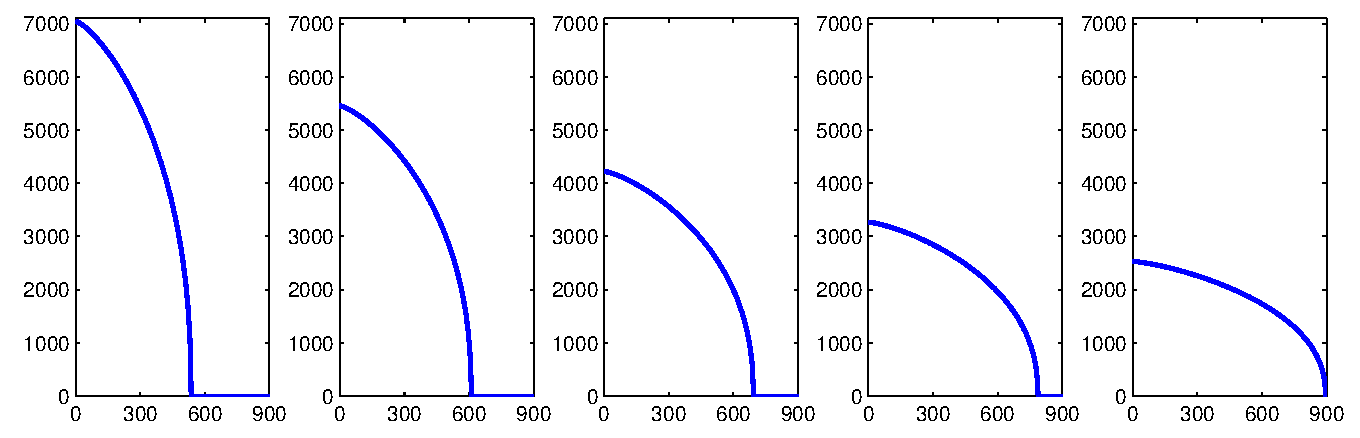
\includegraphics[width=0.95\textwidth]{pdffigs/siascaling}

\medskip
\scriptsize times 1, 10, 100, 1000, 10000 years
\end{center}
\end{frame}


\begin{frame}{similarity solution to the SIA 2}
\label{slide:plothalfar}

\animategraphics[autoplay,loop,height=7.0cm]{4}{anim/halfar}{0}{26}

\par
\scriptsize 
frames from $t=4$ months to $t = 10^6$ years, equal spaced in \emph{exponential} time
\end{frame}


\begin{frame}{similarity solution to the SIA 3}

\begin{itemize}
\item for $n=3$ the solution is:
  $$H(t,r) = H_0 \left(\frac{t_0}{t}\right)^{1/9} \left[1 - \left(\left(\frac{t_0}{t}\right)^{1/18} \frac{r}{R_0}\right)^{4/3}\right]^{3/7}$$
where
  $$t_0 = \frac{1}{18 \Gamma} \left(\frac{7}{4}\right)^3 \frac{R_0^4}{H_0^{7}}$$
and $H_0$, $R_0$ are central height and ice cap radius at $t=t_0$
\item you choose $H_0$ and $R_0$, and these determine the ``characteristic'' time $t_0$
\end{itemize}

\begin{center}
\tiny  more on this in [Nye, 2000] and [Bueler and others, 2005]
\end{center}
\end{frame}


\begin{frame}{finding Halfar solution}

\small
\emph{the method is the same as that which found the fundamental solution of the heat equation}:
\mode<presentation>{\scriptsize}
\begin{itemize}
\item allow scaling of the input and output:\qquad  $s = t^{-\beta} r$, \quad $H(t,r) = t^{-\alpha} \varphi(s)$
\item insert into $H_t = \Div \left(\Gamma H^{5} |\grad H|^{2} \grad H \right)$ \qquad\qquad ($\leftarrow$ \emph{$n=3$ case for simplicity})
\item to eliminate $t$ from the equation, choose $\boxed{7\alpha + 4\beta = 1}$; get
	$$-\alpha \phi - \beta s \varphi' = s^{-1} \left(\Gamma s \varphi^5 |\varphi'|^2\varphi'\right)'$$
\item to write as equality of derivatives, choose $\boxed{-\alpha + 2\beta=0}$:
	$$\left(-\beta s^2 \varphi\right)' = \left(\Gamma s \varphi^5 |\varphi'|^2\varphi'\right)'$$
\item integrate this and use finiteness of $\varphi(0)$, $\varphi'(0)$, and use $\varphi'(s)\le 0$, to get separable ODE
	$$\beta s = \Gamma \varphi^4 (-\varphi')^3$$
\item suppose $H(t_0,0)=H_0$ for some $t_0>0$ to find formula
	$$\varphi(s)^{7/3} = (t_0^\alpha H_0)^{7/3} - \frac{7}{4} \left(\frac{\beta}{\Gamma}\right)^{1/3} s^{4/3}$$
\item write as formula for $H(t,r)$, on previous slide, by solving boxed equations above to get $\alpha=1/9$, $\beta = 1/18$
\item margin location equation $\phi(t_0^{-\beta} R_0)=0$ gives formula for $t_0$ on previous slide
\mode<article>{
\item cases $n\ne 3$, isostatic bed shape, and $M\ne 0$ generalizations in [Bueler and others, 2005]
}
\end{itemize}
\end{frame}


\begin{frame}{evaluating Halfar solution}

\minput{halfar}

\begin{itemize}
\item it is easy to compute it, so \dots
\item \emph{please} use it to verify SIA codes, o.k.?
\end{itemize}
\end{frame}


\begin{frame}{is the Halfar solution \emph{good for any modeling}?}

\begin{itemize}
\item Nye and others [2000] compared the long-time consequences of different flow laws for the South Mars Polar Cap
\item they compared the long-time behavior of the corresponding \emph{Halfar solutions} for the different flow laws, with both $\text{CO}_2$ ice and $\text{H}_2\text{O}$ ice parameters
\item conclusions:
  \begin{quote}
  \dots none of the three possible [$\text{CO}_2$] flow laws will allow a 3000-m cap, the thickness suggested by stereogrammetry, to survive for $10^7$ years, indicating that the south polar ice cap is probably not composed of pure $\text{CO}_2$ ice \dots the south polar cap probably consists of water ice, with an unknown admixture of dust.
  \end{quote}
\item in 2008, NASA's Phoenix lander found water ice in the north polar cap on Mars
\end{itemize}
\end{frame}


\begin{frame}{on \textsl{degenerate} diffusivity}

\begin{itemize}
\item recall that the SIA is
\small
	$$H_t = M + \Div \left(D\, \grad h \right) \quad \text{where} \quad D = \Gamma H^{n+2} |\grad h|^{n-1}$$
\normalsize
\item ``degeneracy'' of $D$ happens in two ways:

\bigskip
\small
\begin{tabular}{l|c|c}
 & why $D\to 0$ & so what? \\ \hline
domes    & $\grad h \to 0$ & \begin{tabular}{c}
$H$ and $\grad h$ are continuous \\ but $\grad^2 h$ is singular
\end{tabular} \\ \hline
margins  & $H \to 0$       & \begin{tabular}{c}
$H$ is continuous \\ but $\grad h$ is singular
\end{tabular}
\end{tabular}
\normalsize
\bigskip

\item numerically, \emph{margins are worse than domes}
\item degenerate diffusion equations are free boundary problems
\item transformation $\eta = H^{(2n+2)/n}$ is known to help \dots for flat beds
\item as a practical matter, numerical solvers for the SIA must handle $u_t = M + \Div \left(D\, \grad u\right)$ for \emph{very} general diffusivity
\end{itemize}
\end{frame}


\begin{frame}
  \frametitle{computing diffusivity in SIA}

\begin{columns}
\begin{column}{0.6\textwidth}
\begin{itemize}
\item for numerical stability we want $D = \Gamma H^{n+2} |\grad h|^{n-1}$ on the staggered grid
\item various schemes proposed; stencil for Mahaffy [1976] scheme at right
\item all schemes involve
  \begin{itemize}
  \item[$\circ$] averaging $H$
  \item[$\circ$] differencing $h$
  \item[$\circ$] in a ``balanced'' way, for better accuracy,
  \end{itemize}
to put $D$ on the staggered grid
\end{itemize}
\end{column}

\begin{column}{0.4\textwidth}
  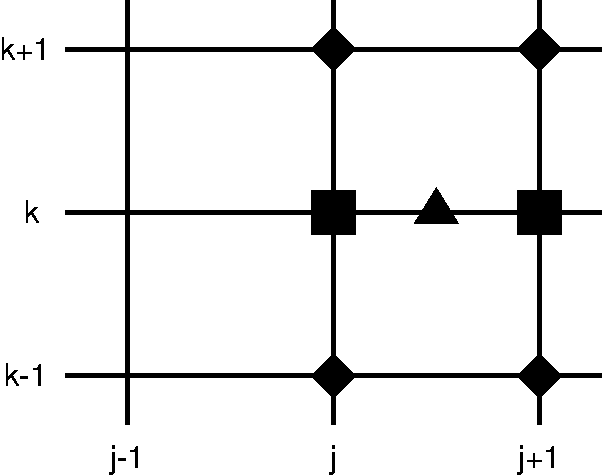
\includegraphics[width=1.0\textwidth]{photos/mahaffystencil}
\end{column}
\end{columns}
\end{frame}


\begin{frame}
  \frametitle{SIA implementation: flat bed case}

\minput{siaflat}
\end{frame}


\begin{frame}{the worst ice sheet}

\begin{itemize}
\item adaptive time-stepping works: \texttt{siaflat.m} takes short time steps when the driving stress $\rho g H |\grad h|$ is large, and then longer steps when it is ``easier''
\item for example, a worst-case ice sheet is \emph{thick} but with a \emph{very bumpy surface}
\item \texttt{roughice.m} generates initial ice sheet, which is thick and with a white-noise surface, then runs for 50 years
\item initial surface, final surface, and time-steps shown below
\end{itemize}

\begin{center}
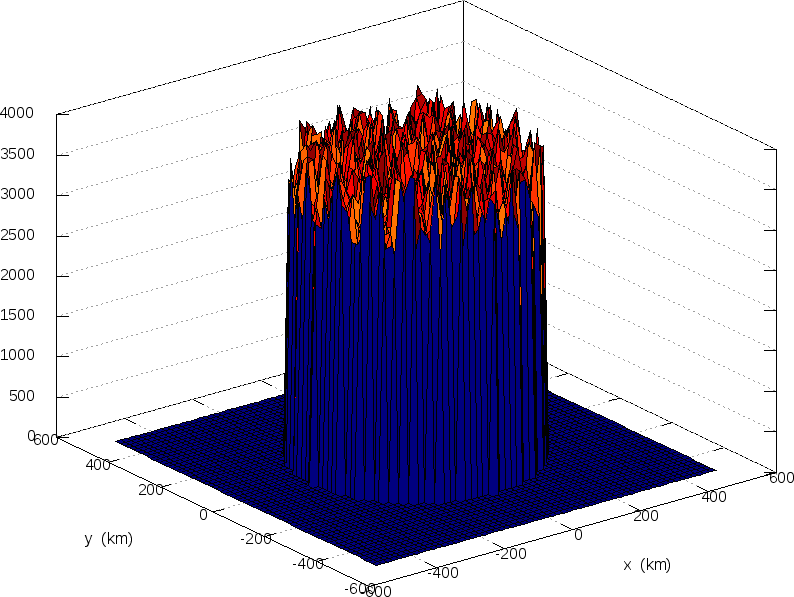
\includegraphics[width=0.3\textwidth]{photos/roughinitial}  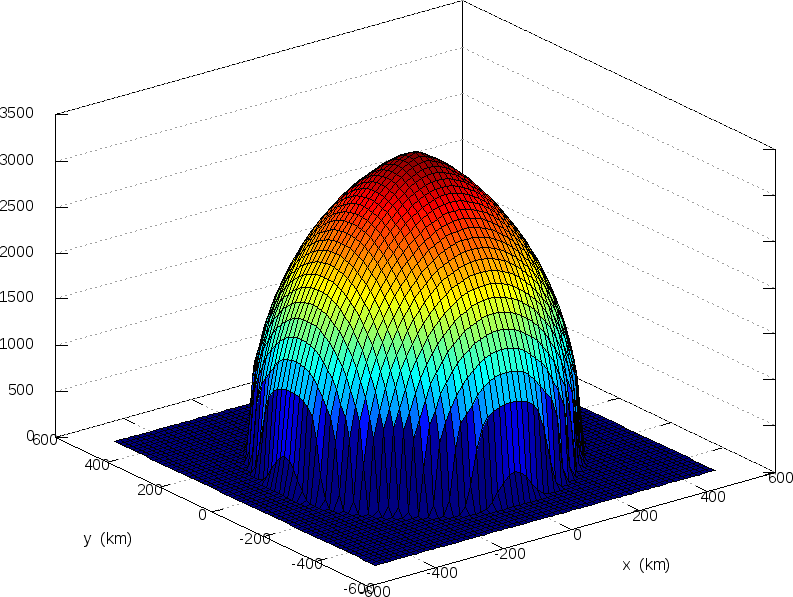
\includegraphics[width=0.3\textwidth]{photos/roughfinal} 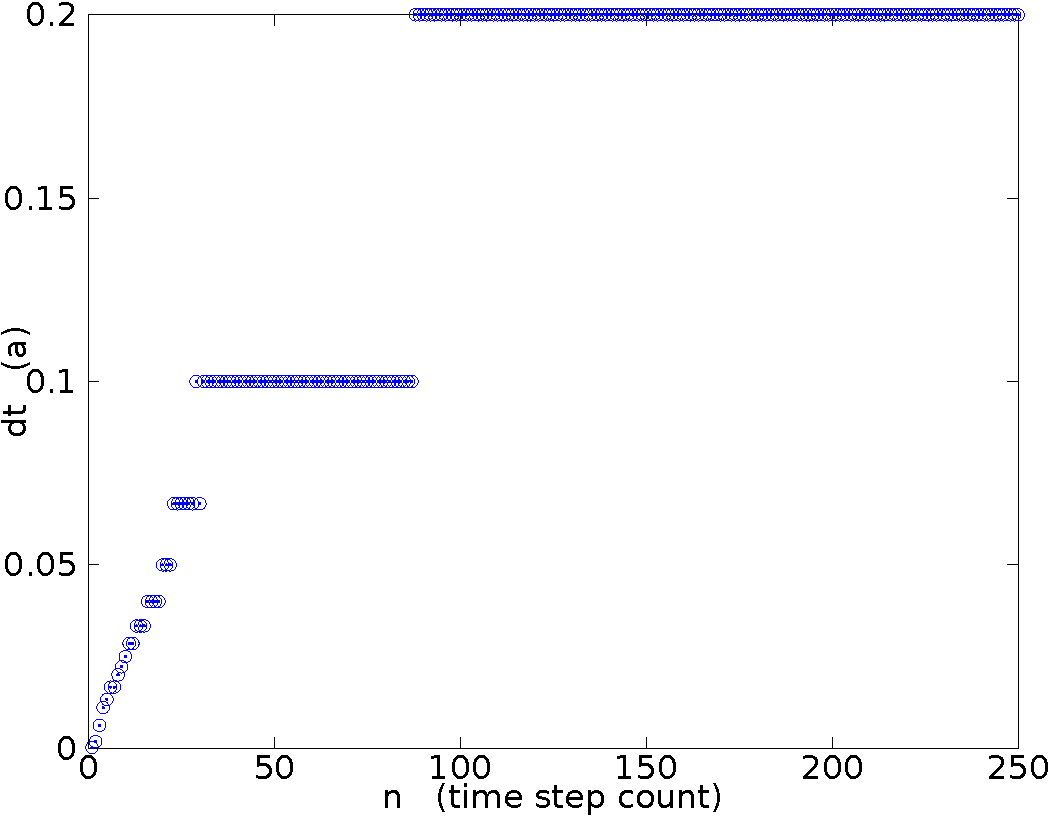
\includegraphics[width=0.38\textwidth]{photos/roughtimesteps}
\end{center}
\end{frame}


\subsection{is it right?}

\begin{frame}{verification of numerical ice flow codes}
\begin{itemize}
\item how do we make sure a numerical scheme \emph{and its implementation} are right?  some available \emph{techniques}
  \begin{enumerate}
  \item  don't make any mistakes
  \item  ``eyeball'' the results when you change the code \dots if it looks right it is right
  \item  from the beginning, build-in a comparison to an exact solution (= verification)
  \end{enumerate}
\end{itemize}
\end{frame}


\begin{frame}[fragile]
\frametitle{verifying our SIA code \texttt{siaflat.m}}

\begin{columns}
\begin{column}{0.6\textwidth}
\minputtiny{verifysia}
\end{column}

\begin{column}{0.4\textwidth}
\small
\begin{itemize}
\item this code calls \texttt{siaflat.m}
\item with initial condition which is a $t_1$ Halfar solution
\item numerical code runs to later time $t_2$ and the compares to Halfar at $t_2$
\end{itemize}

\bigskip
\scriptsize
map of thickness error from

\qquad \texttt{>> verifysia(160,3.0)}:

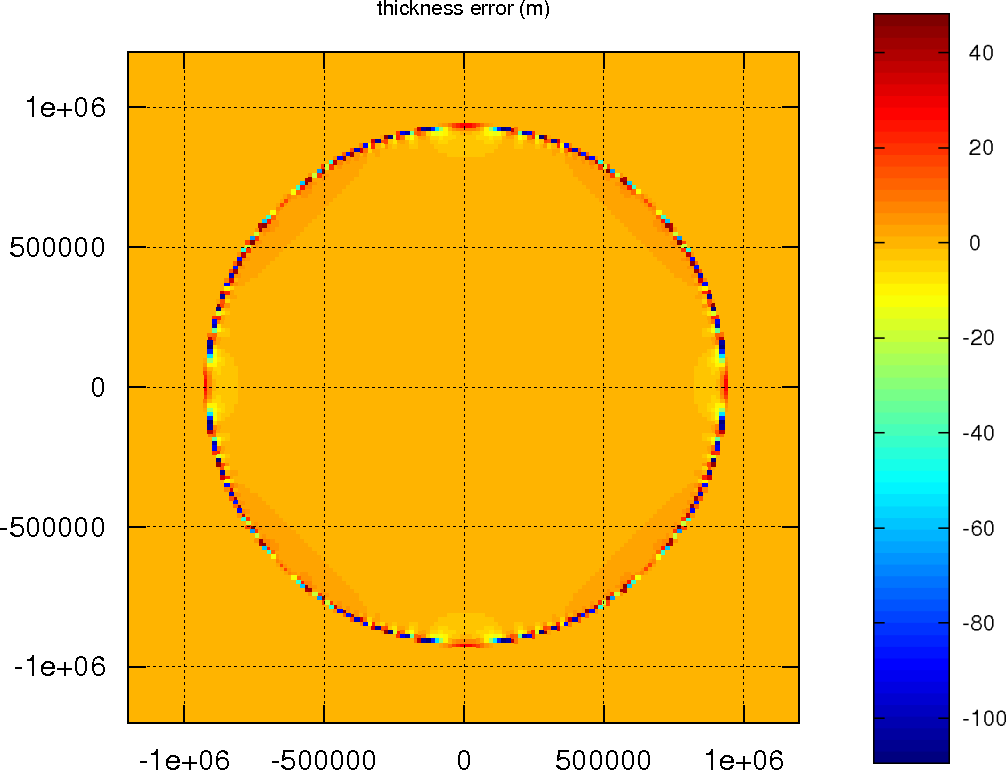
\includegraphics[width=1.0\textwidth]{photos/siaerror}
\end{column}
\end{columns}
\end{frame}


\begin{frame}[fragile]
\frametitle{verifying our SIA code 2}

\begin{columns}
\begin{column}{0.65\textwidth}
\small
\begin{verbatim}
>> verifysia(20,24.0);
errors for 20 x 20 grid:
average thickness error  = 22.335
maximum thickness error  = 227.275
>> verifysia(40,12.0);
errors for 40 x 40 grid:
average thickness error  = 9.519
maximum thickness error  = 241.040
>> verifysia(80,6.0);
errors for 80 x 80 grid:
average thickness error  = 2.937
maximum thickness error  = 159.442
>> verifysia(160,3.0);
errors for 160 x 160 grid:
average thickness error  = 0.988
maximum thickness error  = 103.456
>> verifysia(200,2.0);
errors for 200 x 200 grid:
average thickness error  = 0.827
maximum thickness error  = 94.561
\end{verbatim}
\normalsize
\end{column}

\begin{column}{0.35\textwidth}
\small
\emph{Trust but verify.}
\medskip

\tiny (Ronald Reagan)

\bigskip\bigskip\bigskip

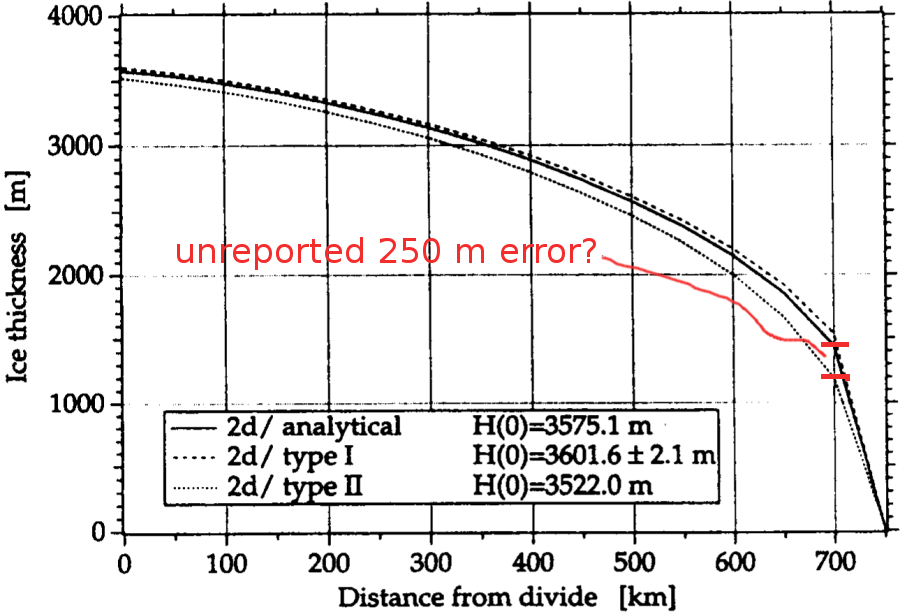
\includegraphics[width=0.95\textwidth]{photos/eismintone}

\scriptsize \emph{figure 2 in [Huybrechts and others, 1996]}
\end{column}
\end{columns}
\end{frame}


\begin{frame}[fragile]
\frametitle{numerical mass conservation}

\begin{itemize}
\item in addition to measuring geometry errors, we might want a numerical code not to lose mass!
\item again, \emph{the Halfar solution is a perfect tool}
  \begin{itemize}
  \item[$\circ$] because the Halfar exact solution has exact (continuum) volume conservation
  \end{itemize}
\item add numerical volume calculation to \texttt{verifysia.m}:
\small
\begin{verbatim}
>> verifysia(20)
vol1       =  3.96112407720492e+15
...
vol2approx =  3.96112407720492e+15
voldiff = 1.50000000000000e+00
\end{verbatim}
\normalsize
\item huh?  how can it be that good?
  \begin{itemize}
  \item[$\circ$] the Mahaffy [1976] scheme has local numerical mass conservation
  \item[$\circ$] but what about the margin where $H\to 0$?
  \item[$\circ$] \texttt{siaflat.m} implements boundary condition \quad ``$H\ge 0$''
  \item[$\circ$] apparently this boundary condition produces global numerical mass conservation to rounding error!
  \end{itemize}
\end{itemize}
\end{frame}


\subsection{application}

\begin{frame}{application to the Antarctic ice sheet}
\small
\begin{itemize}
\item at Karthaus 2009, a computer project: modify \texttt{siaflat.m} to
  \begin{itemize}
  \small
  \item allow arbitrary bed elevation $b(x,y)$
  \item allow arbitrary mass balance $M(x,y)$
  \item apply a marine-margin condition
  \end{itemize}
and then simulate the Antarctic ice sheet
\item my solution: 
  \begin{itemize}
  \small
  \item add 8 lines to \texttt{siaflat.m} in total, creating \texttt{siageneral.m}
  \item use the SeaRISE 5km data set for present-day Antarctica (NetCDF)
  \item add a page or so of code for pre- and post-processing
  \item do 40 ka run starting with present-day geometry
  \end{itemize}
\end{itemize}

\vspace{-0.15in}
\begin{columns}
\begin{column}{0.5\textwidth}
\begin{center}
\scriptsize
initial (observed) surface elevation
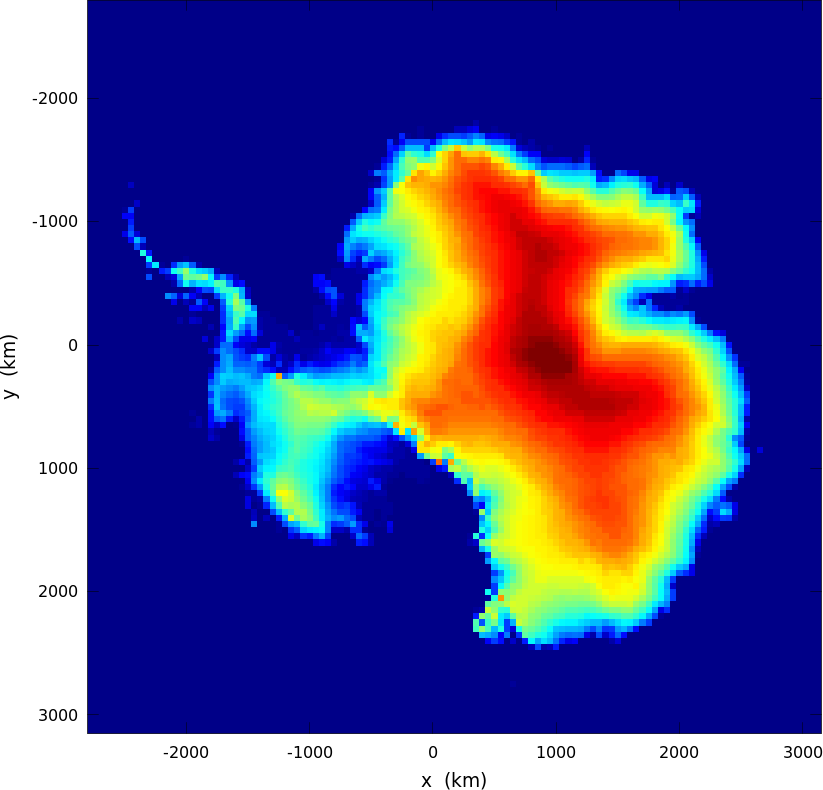
\includegraphics[width=0.8\textwidth]{photos/antinitial}
\end{center}
\end{column}
\begin{column}{0.5\textwidth}
\begin{center}
\scriptsize
40 ka (modeled) surface elevation
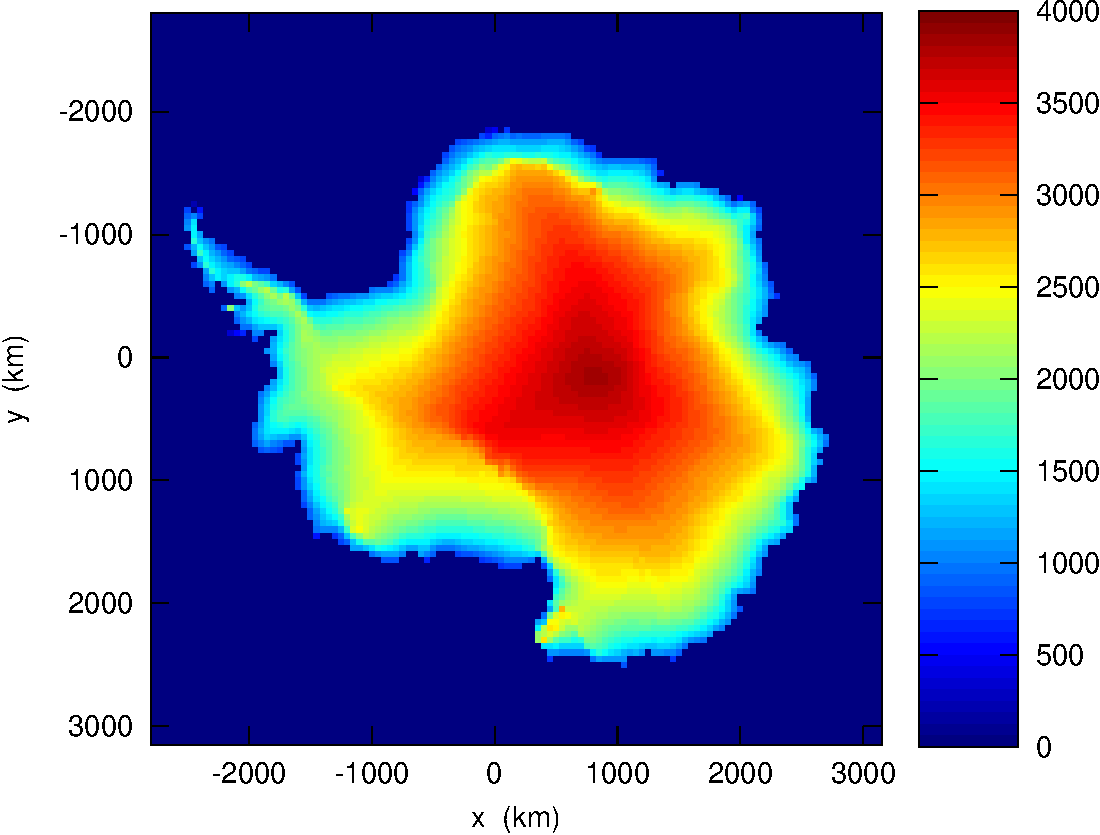
\includegraphics[width=0.8\textwidth]{photos/antfinal}
\end{center}
\end{column}
\end{columns}
\end{frame}


\begin{frame}{application to the Antarctic ice sheet 2}

\begin{columns}
\begin{column}{0.6\textwidth}
\begin{itemize}
\item volume grows
  \begin{itemize}
  \item[$\circ$] levels out at about $33 \times 10^6\,\text{km}^3$
  \item[$\circ$] compare present-day observed volume of $25 \times 10^6\,\text{km}^3$
  \item[$\circ$] exponential time of about 15 ka,
  \item[$\circ$] but exponential time is \emph{much} longer if our model were thermocoupled, because of long advection time-scale  
  \end{itemize}
\end{itemize}
\end{column}
\begin{column}{0.45\textwidth}
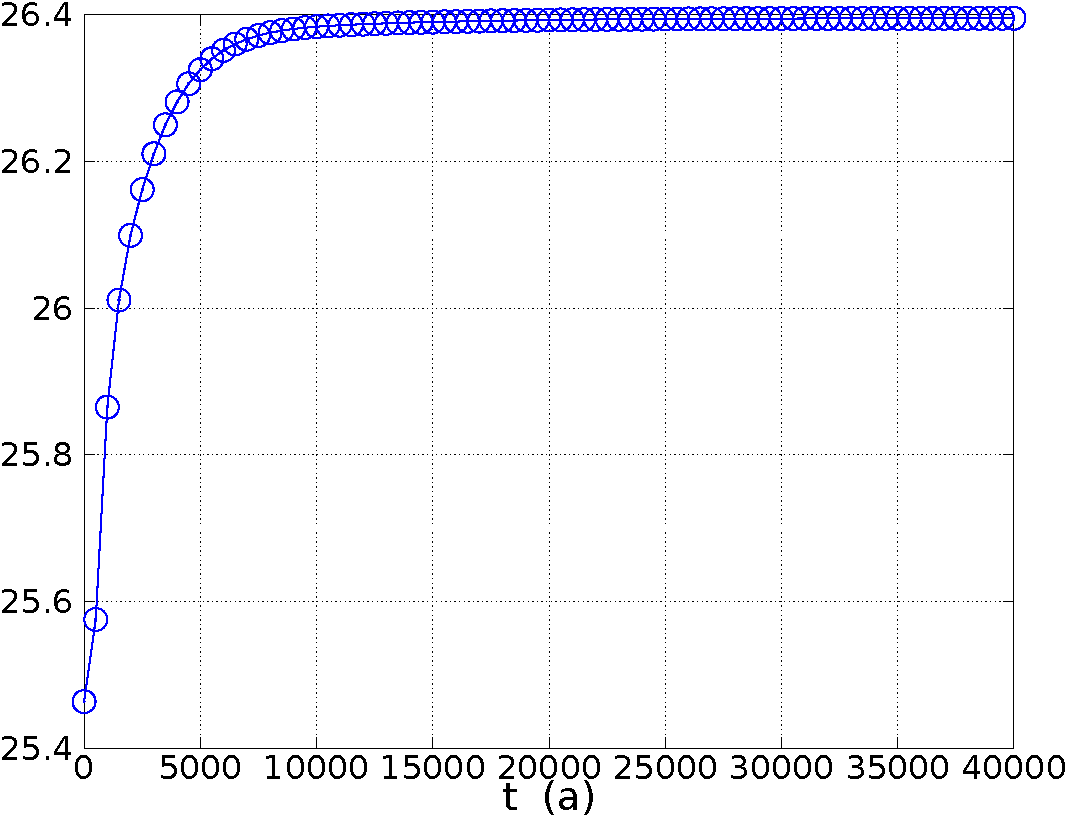
\includegraphics[width=1.0\textwidth]{photos/antvol}
\end{column}
\end{columns}

\begin{itemize}
\item I used $A = 3\times 10^{-16}\,\text{Pa}^{-3}\,\text{a}^{-1}$ 
  \begin{itemize}
  \item[$\circ$] which is an ``enhancement factor'' of 3, \scriptsize relative to the EISMINT I [Huybrechts and others, 1996] value of $A=10^{-16}$ used earlier\small
  \end{itemize}
\item an enhancement factor of 24 would make the volume level out at about the present-day value
\item \emph{pop quiz}:  why is that not a good idea?
\end{itemize}
\end{frame}


\subsection{the most basic shallow assumption}

\begin{frame}{the most basic shallow assumption}

\begin{columns}

\begin{column}{0.6\textwidth}
\begin{itemize}
\item careful derivation of the SIA is next
\item makes ``shallowness assumptions''
\item the most basic is a limitation which applies to \emph{all} shallow ice theories\footnote{\tiny e.g.~SIA, SSA, Blatter-Pattyn, SIA+SSA hybrids, \dots} but not to the general Stokes theory:

\begin{center}
\emph{the surface and base of the ice are given by differentiable functions} $z=h(t,x,y)$ \emph{and} $z=b(t,x,y)$
\end{center}
\item the configurations at right, with overhang in surface, are not allowed
\end{itemize}
\end{column}

\begin{column}{0.4\textwidth}
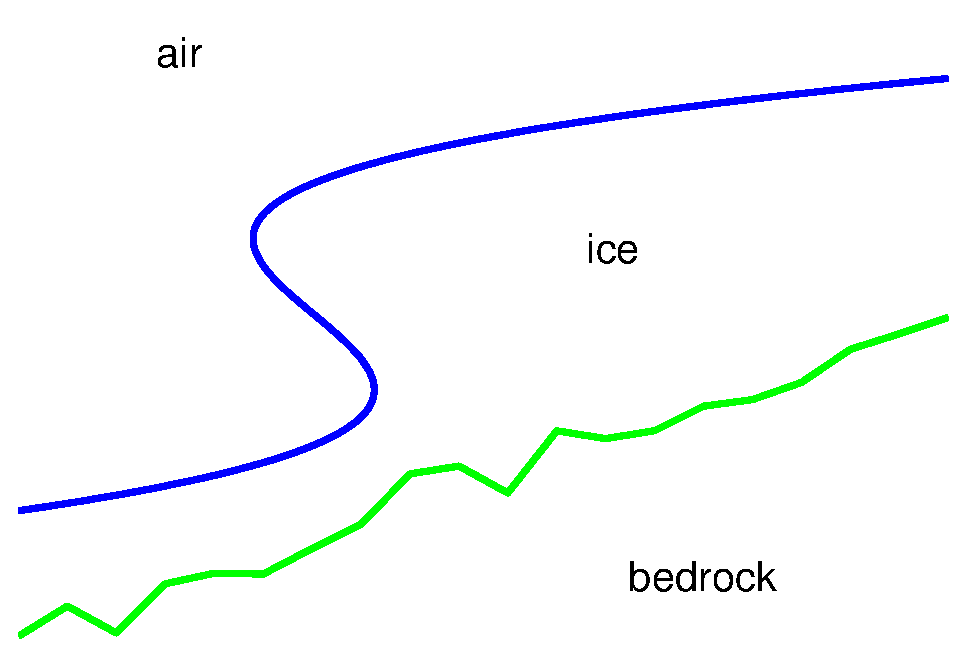
\includegraphics[width=1.0\textwidth]{pdffigs/sshape}
\vspace{20mm}

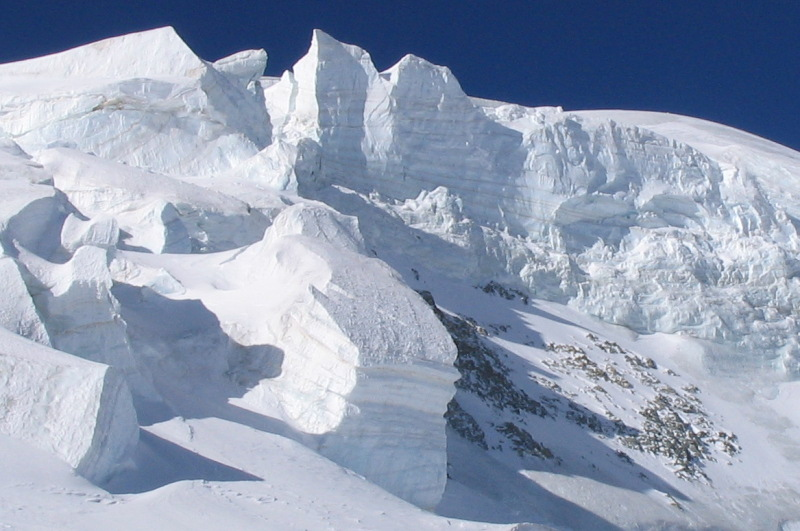
\includegraphics[width=1.0\textwidth]{photos/Serac2}
% uploader was Eltouristo at fr.wikipedia
% Description "sérac sur le galcier blanc qui mène au dôme des écrins avril 2006"
\end{column}
\end{columns}
\end{frame}


\begin{frame}{kinematic and mass continuity equations}

\begin{itemize}
\item what does this ``most basic shallow assumption'' get you?
\item \emph{answer:} a map-plane mass continuity equation
\item consider these three equations:
  \begin{itemize}
  \item[$\circ$]  the surface kinematical equation
  \item[$\circ$]  the base kinematical equation
  \item[$\circ$]  the map-plane mass continuity equation
  \end{itemize}
\item all three equations are important for shallow ice sheets and shelves, but \emph{any two imply the third}
\item the key facts we need:
  \begin{itemize}
  \item[$\circ$]  the incompressibility of ice
    $$u_x + v_y + w_z = 0$$
  \item[$\circ$]  the Leibniz rule for differentiating integrals
  \scriptsize
    $$\frac{d}{dx}\left(\int_{g(x)}^{f(x)} h(x,y)\,dy\right) = f'(x) h(x,f(x)) - g'(x) h(x,g(x)) + \int_{g(x)}^{f(x)} h_x(x,y)\,dy$$
  \end{itemize}
\end{itemize}
\end{frame}


\begin{frame}{kinematic and mass continuity equations 2}

\begin{itemize}
\item let $a$ be the surface mass balance function ($a>0$ is accumulation)
\item let $s$ be the basal melt rate function ($s>0$ is basal melting)
\item define the map-plane flux of ice,
	$$\bq = \int_{b}^{h} (u,v)\,dz = (\bar u, \bar v)\,H$$
\item the three equations are:
\begin{empheq}[left=\text{surface kinematical}\quad,innerbox=\fbox]{equation}
h_t = a - u\big|_h h_x - v\big|_h h_y + w\big|_h  \label{surfkine}
\end{empheq}
\begin{empheq}[left=\text{base kinematical}\quad,innerbox=\fbox]{equation}
b_t = s - u\big|_b b_x - v\big|_b b_y + w\big|_b  \label{basekine}
\end{empheq}
\begin{empheq}[left=\text{mass continuity}\quad,innerbox=\fbox]{equation}
H_t = M - \Div \bq \, \text{ where } M=a-s \label{masscontinuity}
\end{empheq}
\end{itemize}
\end{frame}


\begin{frame}{kinematic and mass continuity equations 3}
\label{slide:twoimplythird}

\small
for example, here is a sketch of how to show \quad \eqref{surfkine} \,\&\, \eqref{basekine} $\implies$ \eqref{masscontinuity}:
\mode<presentation>{\scriptsize}
\begin{enumerate}
\item recalling $H=h-b$ and $M=a-s$, the difference of \eqref{surfkine} and \eqref{basekine} is
\begin{equation}
H_t = M - u\big|_h h_x - v\big|_h h_y + w\big|_h + u\big|_b b_x + v\big|_b b_y - w\big|_b \tag{*}
\end{equation}
\item incompressibility gives difference of surface and base values of $w$ by integration,
\begin{equation}
w_z = - (u_x + v_y) \quad \implies \quad w\big|_h - w\big|_b = - \int_b^h (u_x + v_y)\,d\zeta \notag
\end{equation}
which reduces (*) to: 
\begin{equation}
H_t = M - u\big|_h h_x - v\big|_h h_y + u\big|_b b_x + v\big|_b b_y - \int_b^h (u_x + v_y)\,d\zeta  \tag{**}
\end{equation}
\item on the other hand, the Leibniz rule on $\bq = \int_{b}^{h} (u,v)\,dz$ gives
	$$\Div \bq = u\big|_h h_x + v\big|_h h_y - u\big|_b b_x - v\big|_b b_y + \int_b^h (u_x+v_y)\,dz$$
\item \dots which reduces (**) to
	$$H_t = M - \Div \bq$$
\end{enumerate}
\end{frame}


\begin{frame}{kinematic and mass continuity equations 4}

\begin{itemize}
\item papers have lots of calculations like on the previous slide
\item usually mixed in with other arguments about shallowness
\item most ice sheet models use the mass continuity equation to describe change in ice sheet geometry,
\item \dots but they could instead use the surface kinematical equation
\item in using a stress balance in a shallow theory, all we need to do is get the horizontal velocity $(u,v)$, which gives $\bq$ and thus the mass continuity equation
\item for example, the derivation of the SIA from Stokes needs to only go far enough to find an expression for the horizontal velocity $(u,v)$
\end{itemize}
\end{frame}


\subsection{flowline Stokes}

\begin{frame}{Stokes equations in $x,z$ plane flow case}

\begin{itemize}
\item suppose all flow is in the (screen) $x,z$ plane
\item \dots so out-of-plane velocity is zero ($v=0$) and all quantities are constant in $y$ direction ($\partial/\partial y = 0$)
\item the symmetric strain rate tensor has many zeros
	$$D_{ij} = \frac{1}{2}\left(\frac{\partial u_i}{\partial x_j} + \frac{\partial u_j}{\partial x_i}\right) = \begin{pmatrix}
  	D_{11} & 0 & D_{13} \\
  	0 & 0 & 0 \\
  	D_{13} & 0 & D_{33} \\
  	\end{pmatrix}$$
\item incompressibility of ice in plane flow case says $D$ has trace zero:
	$$u_x + 0 + w_z = D_{11} + D_{33} = 0$$
\item \dots so $D_{33} = - D_{11}$ in this case
\end{itemize}
\end{frame}


\begin{frame}{Stokes equations in $x,z$ plane flow case 2}

\begin{itemize}
\item recall that the Cauchy stress tensor $\sigma_{ij}$, with its pressure part $p$ removed, is called ``deviatoric'':
	$$\tau_{ij} = \sigma_{ij} + p \delta_{ij} \qquad \text{where} \qquad p = -(1/3) (\sigma_{11} + \sigma_{22} + \sigma_{33})$$
\item the deviatoric stress tensor $\tau_{ij}$ is proportional to the tensor $D_{ij}$, in the isotropic (Glen law) case:
	$$D_{ij} = A(T) \tau^{n-1} \tau_{ij}$$
\item \dots where \quad $2 \tau^2 = 2 ({II}_\tau)^2 = \tau_{ij} \tau_{ij}$ \quad so \quad $\tau = \left(\tau_{11}^2 + \tau_{13}^2\right)^{1/2}$
\item so $\tau_{ij}$ is also symmetric, and has trace zero,
\item and $\tau_{ij}$ has only two nonzero entries $\tau_{11}$, $\tau_{13}$:
  	$$\begin{pmatrix}
  	\tau_{11} & 0 & \tau_{13} \\
  	0 & 0 & 0 \\
  	\tau_{13} & 0 & -\tau_{11} \\
  	\end{pmatrix}$$
\end{itemize}
\end{frame}


\begin{frame}{Stokes equations in $x,z$ plane flow case 3}

\begin{itemize}
\item in the 3D case: $n=3$, Glen, isothermal Stokes equations:
\begin{align*}
u_x + v_y + w_z &= 0 \\
0 &= \nabla \cdot \sigma + \rho \mathbf{g} \\
D_{ij} &= A \tau^2 \tau_{ij}
\end{align*}
\item $x,z$ plane flow case: from simplifications on previous slides, the isothermal Stokes equations say
\begin{empheq}[box=\fbox]{align}
u_x + w_z &= 0 \notag \\
p_x &= \tau_{11,x} + \tau_{13,z} \notag \\
p_z &= \tau_{13,x} - \tau_{11,z} - \rho g \label{Stokes} \\
u_x &= A \tau^2 \tau_{11} \notag \\
u_z + w _x &= 2 A \tau^2 \tau_{13} \notag
\end{empheq}
\item five scalar equations in five scalar unknowns ($u,w,p,\tau_{11},\tau_{13}$) but still fairly hard to solve \dots
\end{itemize}
\end{frame}


\begin{frame}{Stokes equations in $x,z$ plane flow case 4}

\begin{itemize}
\item previous equations apply within the ice fluid
\item \dots but \emph{boundary conditions are needed}
\item at the upper surface there is no stress from the air: $\sigma_{ij} n_j = 0$ where $\mathbf{n}$ is a normal vector to the surface
\item in plane flow case use $\mathbf{n} = (h_x,0,-1)$, which is gradient of $F(x,z)=h(x)-z$, which is constant on $z=h(x)$
\item get stress equations at surface:
\begin{align*}
\tau_{13} &= (\tau_{11} - p) h_x \\
p + \tau_{11} + \tau_{13} h_x &= 0
\end{align*}
\item we will only consider non-sliding SIA, so base boundary conditions are
   $$u=0 \quad \text{ and } \quad w=0$$
\end{itemize}
\end{frame}


\subsection{derivation of SIA}


\begin{frame}{scaling the variables}
\label{slide:siascalings}

\begin{itemize}
\item following Chapter 18 of [Fowler, 1997], \emph{Mathematical Models in the Applied Sciences}
  \begin{itemize}
    \scriptsize
    \item which does a much more general job than here: 3D case with conservation of energy, while we only do 2D isothermal case
    \item we also miss Andrew standing on a table and singing, too
    \normalsize
  \end{itemize}
\item consider ice sheet of typical depth $d$ and length $\ell$, and with velocity ($[u]$), deviatoric stress ($[\tau]$), and softness ($[A]$) scales
\item $\eps = d/\ell$ is the ``aspect ratio'' of the ice sheet
\item change to new starred variables using scales:\small
\begin{align*}
x &= \ell\, x^* &         u &= [u] u^* \\
z &= d\, z^*    &         w &= \eps [u] w^* \\
h &= d\, h^*    & \tau_{11} &= \eps [\tau] \tau_{11}^* \\
H &= d\, H^*    & \tau_{13} &= [\tau] \tau_{13}^* \\
A &= [A] A^*  & p - \rho g (h-z) &= \eps [\tau] p^*
\end{align*}
\normalsize
\end{itemize}
\end{frame}


\begin{frame}{scaling the variables 2}

\begin{itemize}
\item we will necessarily choose relations among the scales
\item the choice of such relations affects the outcome and is subject to ``scientific judgment'' (i.e.~controversy)
\item ``\dots the purpose is to attain `properly scaled' equations in which the largest dimensionless parameters are numerically of order one \dots'' [Fowler, 1997]
\item \emph{method}: we rewrite the Stokes equations and the boundary conditions in the newly (starred) variables, \emph{then} check that the scaling relations give reasonable values, \emph{then} remove terms to get a new, more-solvable model, the SIA
\item the scaling relations used here are:
\begin{align*}
\begin{matrix}
\text{balance of shear stress} \\
\text{and pressure gradient}
\end{matrix} && [\tau] &= \rho g d \eps \\
\text{balance of flow law scales} && \frac{[u]}{d} &= 2 [A] [\tau]^3
\end{align*}
\end{itemize}
\end{frame}


\begin{frame}{scaling the equations}

\small
\emph{example}:
\begin{itemize}
\item recall this equation from Stokes equations \eqref{Stokes}:
  $$p_x = \tau_{11,x} + \tau_{13,z}$$
\item replace all variables with their starred versions:
  $$\frac{\eps [\tau]}{\ell} p^*_{x^*}+ \frac{d \rho g}{\ell} h^*_{x^*} = \frac{\eps [\tau]}{\ell} \tau^*_{11,x^*} + \frac{[\tau]}{d}\tau^*_{13,z^*}$$
\item multiply by $\ell / (\eps [\tau])$:
  $$p^*_{x^*}+ \frac{d \rho g}{\eps [\tau]} h^*_{x^*} = \tau^*_{11,x^*} + \frac{\ell}{d \eps}\tau^*_{13,z^*}$$
\item use relation $[\tau] = \rho g d \eps$ and $\eps = d/\ell$:
  $$p^*_{x^*}+ \eps^{-2} h^*_{x^*} = \tau^*_{11,x^*} + \eps^{-2}\tau^*_{13,z^*}$$
\item re-arrange to taste and remove stars:
	$$h_x = \tau_{13,z} + \eps^2 \left(\tau_{11,x} - p_x\right)$$
\item \dots do this for each of the Stokes equations
\end{itemize}
%notes:
% if $f=[f]f^*$ and $x=[x]x^*$ for $f=f(x)$ then $f_x = \frac{[f]}{[x]} f^*_{x^*}$
% the scaling ``$p - \rho g (h-z) = \eps [\tau] p^*$'' implies $p=\eps [\tau]p^* + d \rho g (h^* - z^*)$
\end{frame}


\begin{frame}{scaling the equations 2}

\begin{itemize}
\item Stokes system now appears this way (\emph{stars are removed}):
\begin{align*}
u_x + w_z &= 0 \\
h_x &= \tau_{13,z} + \eps^2 \left(\tau_{11,x} - p_x\right) \\
p_z &= \tau_{13,x} - \tau_{11,z} \\
u_x &= \frac{1}{2} A \left(\eps^2 \tau_{11}^2 + \tau_{13}^2\right) \tau_{11} \\
u_z + \eps^2 w _x &= A \left(\eps^2 \tau_{11}^2 + \tau_{13}^2\right) \tau_{13}
\end{align*}
\item this is still full Stokes!
\item surface conditions are
\begin{align*}
\tau_{13} &= \eps^2 \left(\tau_{11} - p\right) h_x \\
p + \tau_{11} + \tau_{13} h_x &= 0
\end{align*}
\item base conditions are $u=0$ and $w=0$ as before
\end{itemize}
\end{frame}


\begin{frame}{checking the scales}

\begin{itemize}
\item the scale for vertical velocity is already chosen as $\eps [u]$
\item \dots and we now identify this scale with a typical value for accumulation: $[a] = \eps [u]$
\item thus we have chosen these scale relations:
  \begin{align*}
  \eps &= \frac{d}{\ell}           & [\tau] &= \rho g d \eps \\
  \frac{[u]}{d} &= 2 [A] [\tau]^3  &    [a] &= \eps [u]
  \end{align*}
\item to check their reasonableness, we will determine other scale factors in terms of $\ell$, $[a]$, and $[A]$, which are taken from observations:
  $$\ell = 3000\,\text{km},$$
  $$[a] = 0.1\,\text{m}\,\text{a}^{-1}$$
  $$[A] = 2 \times 10^{-16}\,\text{Pa}^{-3}\,\text{a}^{-1}$$
\end{itemize}
\end{frame}


\begin{frame}{checking the scales 2}

\begin{itemize}
\item solving for $d,\eps,[\tau],[u]$ gives
  \begin{align*}
  d &= \left(\frac{\ell^4 [a]}{2 [A] (\rho g)^3}\right)^{1/8} \approx 3600\,\text{m} \\
  \eps &= \frac{d}{\ell} \approx 10^{-3} \\
  [\tau] &= \rho g d \epsilon \approx 4 \times 10^4\, \text{Pa} = 0.4\,\text{bar}\\
  [u] &= 2 [A] d [\tau]^3 \approx 80\,\text{m}\,\text{a}^{-1}
  \end{align*}
\item these are all reasonable values for large ice sheets
\item it is reasonable to proceed to delete terms from the scaled equations to get the reduced (shallow) theory, the SIA
\item the actual measure of the quality of SIA is the comparison of its predictions to observations, when modeling various real ice sheets etc., \emph{not these scalings}
\end{itemize}
\end{frame}


\begin{frame}{finally get to the SIA}
\label{slide:siafinally}

\small
\begin{itemize}
\item setting $\eps=0$ in the scaled Stokes equations, get these equations (left column) and boundary conditions (right):
\begin{align*}
u_x + w_z &= 0                          & \tau_{13}\big|_h &\stackrel{\ast}{=} 0 \\
h_x &\stackrel{\ast}{=} \tau_{13,z}                      & p\big|_h + \tau_{11}\big|_h + \tau_{13}\big|_h h_x &= 0\\
p_z &= \tau_{13,x} - \tau_{11,z}        & & \\
u_x &= \frac{1}{2} A \tau_{13}^2 \tau_{11} & u\big|_b &\stackrel{\dagger}{=} 0 \\
u_z &\stackrel{\dagger}{=} A \tau_{13}^3 & w\big|_b &= 0
\end{align*}
\item combine the two marked ``$\ast$'', integrating vertically from surface $z=h$ to arbitrary elevation $z$, to get
	$$\tau_{13} = - (h - z) h_x$$
\item combine the two marked ``$\dagger$'', integrating vertically from base $z=b$ to arbitrary level $z$, and use the new expression for $\tau_{13}$, to get
\begin{align*}
u(z) &= A \int_b^z \tau_{13}^3\,d\zeta = - A (h_x)^3 \int_b^z (h - \zeta)^3\,d\zeta \\
     &= -\frac{A}{4} (h_x)^3 \left[H^4 - (h - z)^4\right]
\end{align*}

\end{itemize}
\end{frame}


\begin{frame}{finally get to the SIA 2}

\small
\begin{itemize}
\item remember I said that it suffices to find an expression for the horizontal velocity, in order to state the SIA?  \quad \emph{we are there!}
\item the previous slides have been in scaled quantities; now we recall the stars:
   $$u^* = -\frac{A^*}{4} (h^*_{x^*})^3 \left[(H^*)^4 - (h^* - z^*)^4\right]$$
\item and then unscale to find a dimensional expression for $u$, using $h^*_{x^*} = \eps^{-1} h_x$, and using scaling relations:
\begin{align*}
u &= [u] u^* = -\frac{[u] A}{4 [A]} \eps^{-3} (h_x)^3 d^{-4} \left[H^4 - (h - z)^4\right] \\
  &= - \left(\frac{[u]}{4 [A] \eps^3 d^4}\right) A (h_x)^3 \left[H^4 - (h - z)^4\right] \\
  &= - \left(\frac{2 [A] d (\rho g d \eps)^3}{4 [A] \eps^3 d^4}\right) A (h_x)^3 \left[H^4 - (h - z)^4\right] \\
  &= - \frac{1}{2} A (\rho g)^3 (h_x)^3 \left[H^4 - (h - z)^4\right]
\end{align*}
\end{itemize}
\end{frame}


\begin{frame}{finally get to the SIA 3}

\begin{itemize}
\item recall that the flux of ice is $q = \int_b^h u(z) \,dz$
\item so we integrate the expression for $u(z)$:
\begin{align*}
q &= -\frac{1}{2} A (\rho g)^3 (h_x)^3 \int_b^h \left[H^4 - (h - z)^4\right]\,dz \\
  &= -\frac{1}{2} A (\rho g)^3 (h_x)^3 \left[H^5 - \frac{1}{5}(H^5 - 0)\right] \\
  &= -\frac{2}{5} A (\rho g)^3 (h_x)^3 H^5
\end{align*}
\item the mass continuity equation now says:
\begin{align*}
H_t &= M - q_x = M + \left(\frac{2}{5} A (\rho g)^3 (h_x)^3 H^5\right)_x \tag{$\ast$}
\end{align*}
\item equation ($\ast$) matches equation \eqref{sia} in the plane flow case
\end{itemize}
\end{frame}


\begin{frame}{have I oversold diffusivity?} 

\begin{itemize}
\item I have asserted that the default model for ice sheets, the SIA, is a \emph{diffusion}
\item recall the analogy:

\bigskip
\begin{tabular}{ccc}
\emph{diffusion eqn} & $\leftrightarrow$ & \emph{SIA} \\ \hline
$u_t = \Div\left(D \grad u\right)$ & $\leftrightarrow$ & $h_t = M + \Div\left(D \grad h\right)$ \\
$D=D(x,y)$ & $\leftrightarrow$ & $D = \Gamma H^{n+2} |\grad h|^{n-1}$ \\
\end{tabular}

\bigskip
\item have I oversold this diffusivity analogy?
  \begin{itemize}
  \item[$\circ$] probably
  \item[$\circ$] \dots and I've acknowledged there are ``issues''
  \end{itemize}
\item but it turns out there is some robustness to my analogy
  \begin{itemize}
  \item[$\circ$] as follows on the next two slides
  \end{itemize}

\end{itemize}
\end{frame}


\begin{frame}{have I oversold diffusivity? 2}

\emph{DIFFUSIVE IDEA 1}: rough beds have the effect of \emph{reducing} diffusivity
\begin{itemize}
\item define the local bed topography by removing the local mean over some range $\lambda \approx 10$ km:
\small
   $$\tilde b(x,\xi) = b(x+\xi) - \fint_{-\lambda}^\lambda b(x+\xi)\,d\xi$$
\normalsize
\item define this strange average of the local bed:
\small
	$$\theta(x) = \left(\fint_{-\lambda}^\lambda \left(1 - \frac{\tilde b(x,\xi)}{H(x)}
                           \right)^{-(n+2)/n}\,d\xi\right)^{-1/n}$$
\normalsize
\item using a multiple-scales analysis, Schoof [2003] says you will get closer to solving the Stokes equations by making these two modifications of the SIA:
  \begin{itemize}
  \item[$\circ$] smooth the bed, \qquad \tiny \emph{(modelers want to do that anyway)} \small
  \item[$\circ$] but don't lose track of the smoothed-away local bed roughness; use it to reduce the diffusivity:
  \small
  		$$D_{\text{new}} = \theta D \qquad \text{where } 0 \le \theta \le 1$$
  \end{itemize}
\end{itemize}
\end{frame}


\begin{frame}{have I oversold diffusivity? 3}

\emph{DIFFUSIVE IDEA 2}: the large-scale effect of sliding in ice streams (\emph{addressed in next section}), is diffusive
\begin{itemize}
\item suppose that, for an ice stream modeled by the SSA equation
   $$\left(2 A^{-1/n} H |u_x|^{1/n - 1} u_x \right)_x - C|u|^{m-1}u = \rho g H h_x$$
we assume that the basal resistance term balances the driving stress:
   $$- C|u|^{m-1}u = \rho g H h_x$$
\item then the ice stream geometry evolves by a diffusion,
	$$h_t = M + \Div\left(D\,\grad h\right) \qquad \text{where } D = C' H^{(1/m)+1}|\grad h|^{(1/m)-1}$$
\item this ``outer problem'' is part of a matched asymptotic expansion that \emph{does a good job of tracking the grounding line in a marine ice sheet} [Schoof, 2007]
\end{itemize}
\end{frame}
